\section{Strongly Anisotropic Systems}
\label{ch:anis}

By now it should be clear that the notion of scale invariance is a central
tenet of the modern critical phenomena narrative. Several critical systems
however are explicitly not scale invariant in its strictest sense, systems that
have different properties depending on the direction in which you're looking,
that is, they're \textit{anisotropic}. Anisotropy can arise due to the presence
competing interactions, stratified structures or simply due to the system being
out of equilibrium.

One can easily induce anisotropy in a model by introducing asymmetric
interactions, for example you could take the Ising model with different
coupling parameters $J_\parallel$ and $J_\perp$ for different directions. These
types of anisotropy however can be removed by the rescaling of one of the axes.
Such systems are called weakly anisotropic. On the other hand, there are
systems that cannot have their anisotropy removed by rescaling of the axes, in
fact rescaling only exacerbates the anisotropy. These are called
\textit{strongly anisotropic} systems, and they present a significant, and
often overlooked, challenge to those studying critical systems. That's because
these systems are not scale invariant \textit{per se}, so most of the results
shown in Section~\ref{sec:scaling} do not translate well into these systems.
We can, however, assume that they are invariant under an \textit{anisotropic}
scale transformation. This means that the correlation functions transform like
\begin{equation}
    C\left(\mathbf{r}\right)=
    C\left(\mathbf{r}_{\parallel},\mathbf{r}_{\perp}\right)=
    b^{2x}C\left(b\mathbf{^{\theta}r}_{\parallel},b\mathbf{r}_{\perp}\right)
\end{equation}
where $\mathbf{r}=\mathbf{r}_{\parallel}+\mathbf{r}_{\perp}$ and the vector
$\mathbf{r}_{\parallel}$ and $\mathbf{r}_{\perp}$
is a preferential direction (normally assumed to be the time, but it could be a
spatial coordinate without loss of generality). The exponent $\theta$ is
universal and called \textit{anisotropic exponent}, and it basically quantifies
the asymmetry between the directions.

Because the correlation functions are asymmetric, the critical exponents
associated with it also have two different values $\eta_\parallel$,
$\eta_\perp$. The anisotropic exponent relate to them through the relation
\begin{equation}
    \theta = \frac{\eta_\parallel}{\eta_\perp}.
\end{equation}
The correlation length also scales differently in each direction
\begin{equation}
    \xi_{\parallel}=
    \left|T-T_{c}\right|^{-\nu_{\parallel}},
    \,\,\,\,\,\,\,
    \xi_{\perp}=\left|T-T_{c}\right|^{-\nu_{\perp}}
\end{equation}
In dynamical phase transitions, where $\mathbf{r}_\parallel$ plays the role of
time $t$, we also find the new scaling law
\begin{equation}
    \xi_{\perp}\left(t\right)=t^{1/z},
\end{equation}
where
\begin{equation}
    z = \frac{\nu_\parallel}{\nu_\perp},
\end{equation}
which is called as the \textit{dynamical exponent}.

Some effort has been put in order to study.~\cite{Henkel1994}.

%It has been determined that if $\theta = 2/N$, where $N$ is a positive integer,
%the systems if invariant under local scale invariance [???], which is the same
%principle that motivated the introduction of conformal invariance (which is in
%fact the case $N=2$). This observation have been used to successfully study
%some anisotropic systems, like the Liftshitz point in the ANNNI [???] and
%spherical models [???].


\subsection{Multi-Layered Percolation}
\label{sec:mlp}

The percolation model as presented in Section~\ref{sec:perc} was initially
motivated by transport in disordered media, like porous rocks. However, the
morphology of earth's crust is highly non-uniform and
anisotropic~\cite{Englman1986}, such as the case of stratified rocks formed by
the layered deposition of different types of sediment, each with have different
physical properties such as density and porosity. This layered arrangement have
a significant influence in the transport properties of these rocks. Aiming to
model the structure of these kind of media, Dayan \textit{et
al.}~\cite{Dayan1991} introduced yet another variant of the percolation
model, called multi-layered percolation. 

In this model we take a $d$-dimensional lattice composed of several
$(d-1)$-dimensional sub-lattices (or layers) arranged in sequence as if they're
stacked one over the other. Following convention, we'll call the axis
perpendicular to the layers the $y$-axis. We then perform the usual percolation
process by randomly occupying the lattice sites. The key difference here is
that each layer has its own occupation probability $p(y)$. For simplicity, it
is common to take a two-probability approach, where each layer can have one of
two values $p_1$ and $p_2$. These are the control parameters of the model,
where the line $p_1=p_2$ represents the regular isotropic percolation. The
larger the difference between $p_1$ and $p_2$ the more accentuated is the
anisotropy of the systems. To make this more evident it is common to redefine
the control parameters by taking
\begin{equation}
    \bar{p}=\frac{p_1 + p_2}{2},\;\;\;\;\;\;\;\Delta=\frac{p_1 - p_2}{2}
\end{equation}
such that $p_1 = \bar{p} + \Delta$ and $p_2 = \bar{p} - \Delta$. The parameter
$\Delta$ can take any value in the interval $[0.0,0.5]$, and represents the
degree of anisotropy of the system, where the system falls back to the
isotropic case when $\Delta=0$. See Figure~\ref{fig:mlperco_explain} for an
illustration of the multi-layered percolation process. Figure~\ref{fig:mlperco}
shows three realizations of the model for three different values of $\Delta$.
The anisotropy can get very extreme, to the point where it's difficult to
visualize the clusters. In Figure~\ref{fig:mlp_cluster} we used the
self-organized percolation algorithm~\cite{Parteli2010} to generate individual
clusters of multi-layered percolation.

Just like isotropic percolation, the multi-layered version also undergoes a
second-order phase transition from a non-percolated to a percolated phase. The
order parameter  remains the same (the relative size of the largest cluster),
but now we have two control parameters, $p$ and $\Delta$, so instead of a
critical point we have a critical line separating the two phases, as you can
see in the phase diagram show in Figure~\ref{fig:mlp_ps0}. In the case
$\Delta=0$ the value of $p_c$ found is around $0.592$ which is the same as
isotropic percolation as expected, but it falls continuously to $p_c=0.5$ as
$\Delta\rightarrow 0.5$.

Because actually generating clusters of multi-layered percolation can be a
complicated matter and the model has no analytical solution, the critical
properties of multi-layered percolation were determined numerically through
analysis of the cluster perimeters~\cite{Dayan1991, Samyr2009}. This is done by
generating cluster perimeters in a finite lattice, each perimeter defined by
sequence of $N$ points at positions $\mathbf{r}_i=X_i\mathbf{x}+Y_i\mathbf{y}$.
The root means square of the displacement in each direction
\begin{equation}
    F_{X}\left(n\right)=
    \sqrt{\frac{1}{N-n}\sum_{i}{\left(X_{i+n-1}-X_{i}\right)}^{2}},
\end{equation}
(and analogously for $Y$) scales like
\begin{equation}
    F_{X}\left(n\right)\sim n^{-\bar{\nu}_{x}},
    \,\,\,\,\,\,\,\,\,
    F_{Y}\left(n\right)\sim n^{-\bar{\nu}_{y}}.
\end{equation}
The exponents $\bar{\nu}_i$ relate to the actual $\nu_i$ though the relation
\begin{equation}
    \bar{\nu}_i = \nu_i \bar{\sigma}
\end{equation}
where $\bar{\sigma}$ is defined similarly as the $\sigma$ given in
Eq.~\ref{eq:sig}, but for perimeter lengths instead of cluster sizes.
What was found is that as $n\rightarrow\infty$, the $\bar{\nu}_i$ are
independent of $\Delta$ (as long as it is larger that zero).
This means that all the $\Delta$ belong to the same universality class
with $\bar{\nu}_x=0.94\pm0.01$ and $\bar{\nu}_y=0.21\pm0.01$, and
indicates that $\nu_x=13/6$ and $\nu_y=1/2$.

%As is expected, this model presents a second-order phase transition.
%To determine the $\bar{p}_c(\Delta)$, Dayan et al.\ made use of the
%cluster perimeter method.

%We generate various cluster perimeters using the exploration method described
%in Sec.~[???]. Making use of the fact that at the critical point a cluster
%perimeter have equal chances of being an external or an internal border. We
%generate several cluster perimeter and count the ration $R(\bar{p}, \Delta)$
%between the number of realizations where the path was an internal perimeter and
%the number of realizations where it was an external perimeter. The critical
%point is such that $R(\bar{p}_c, \Delta_c)=1$. In the case of a square lattice
%(the one studied by Dayan), we observe that there is a function
%$\bar{p}_c(\Delta)$ that defines the border between the percolating and
%non-percolating phases. This result can be seen in Fig.~[???]. Somewhat
%surprisingly the same method was performed for the triangular lattice, and we
%observed that $\bar{p}_c=0.5$ independent of the value of $\Delta$.

\begin{figure}
\begin{center}
    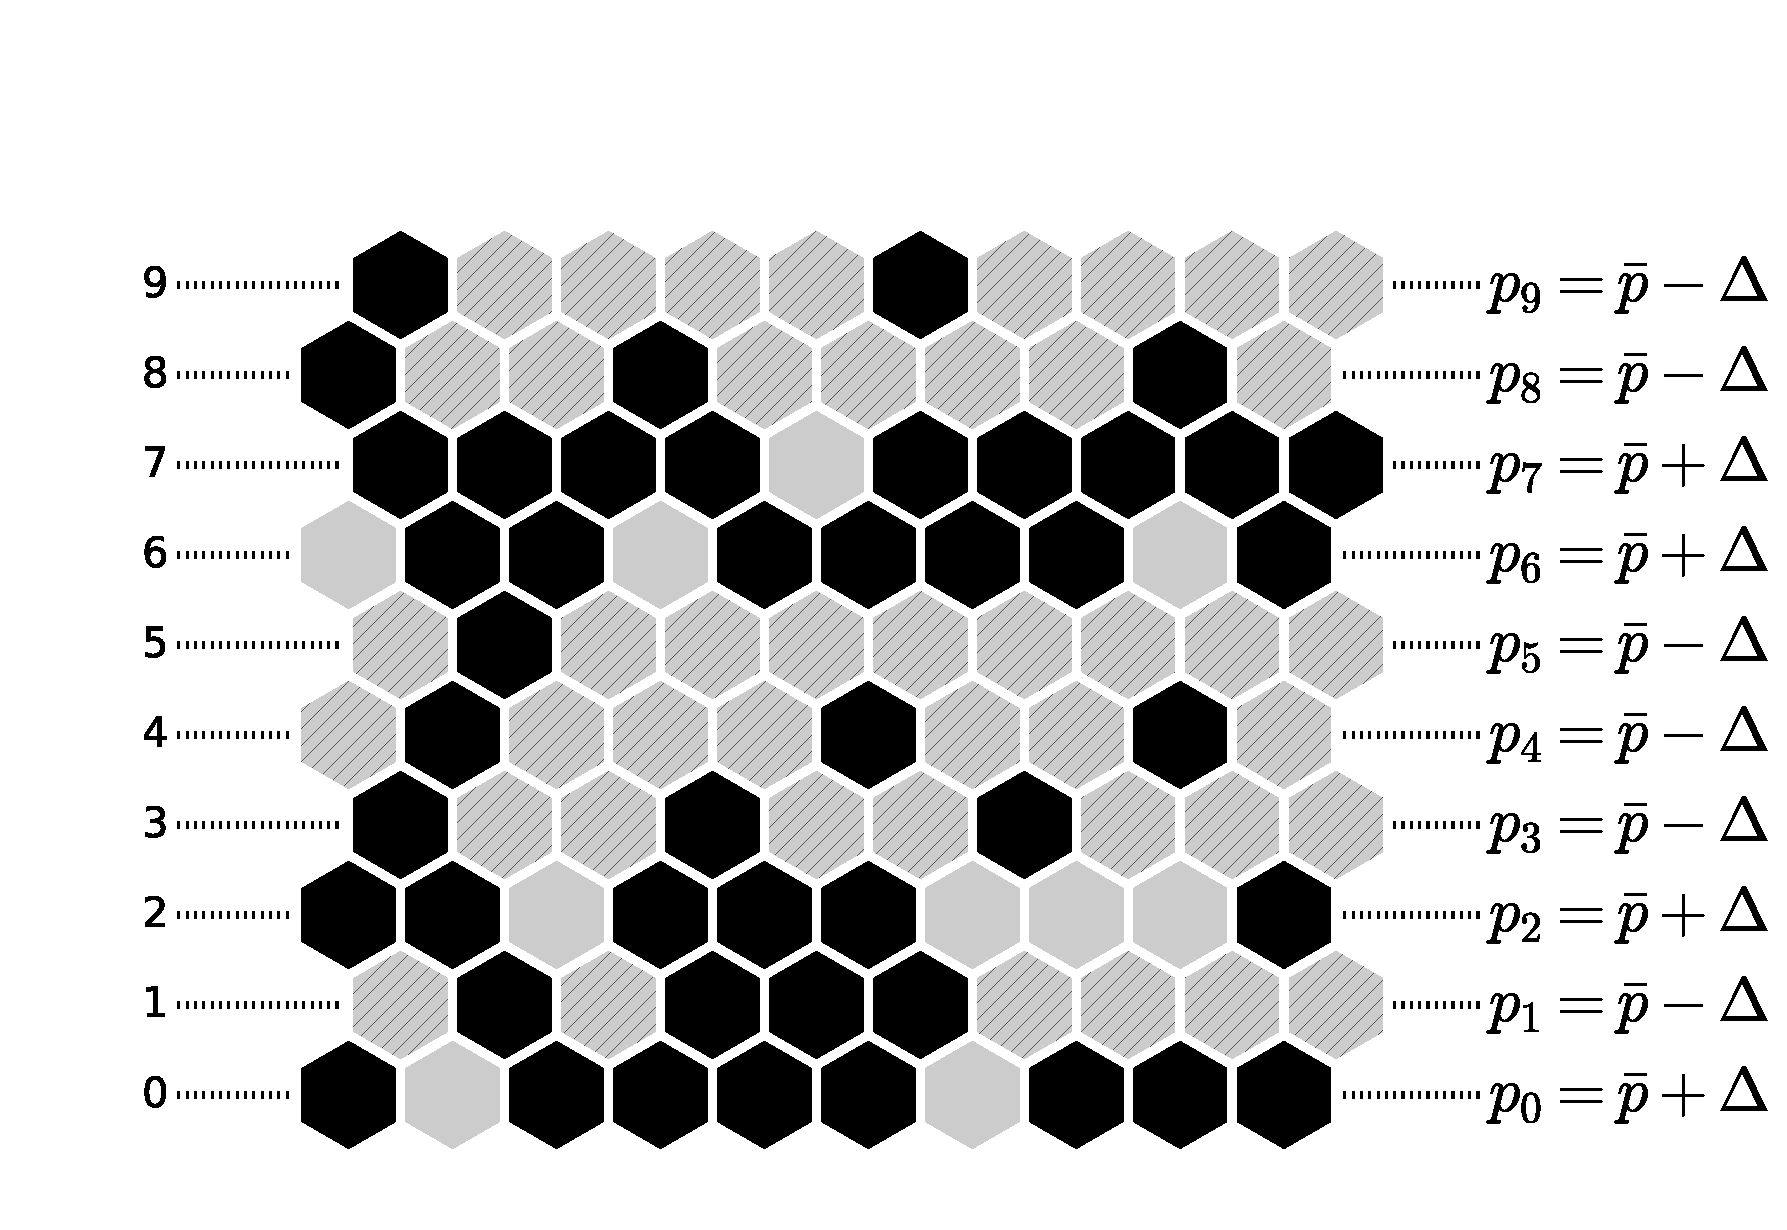
\includegraphics[scale=0.4]{chapters/ch5-anis/figs/mlperco_explain}
\end{center}
\caption{Schematic representation of the multi-layered percolation model. Each
    layer (numbered $0$ through $9$ here) gets one of two probabilities of
    occupation ($\bar{p}\pm\Delta$), chosen randomly with equal probabilities.
    Otherwise, the percolation process goes as usual, occupying each site
    according to the probabilities of each layer.}
\label{fig:mlperco_explain}
\end{figure}

\begin{figure}
\begin{center}
    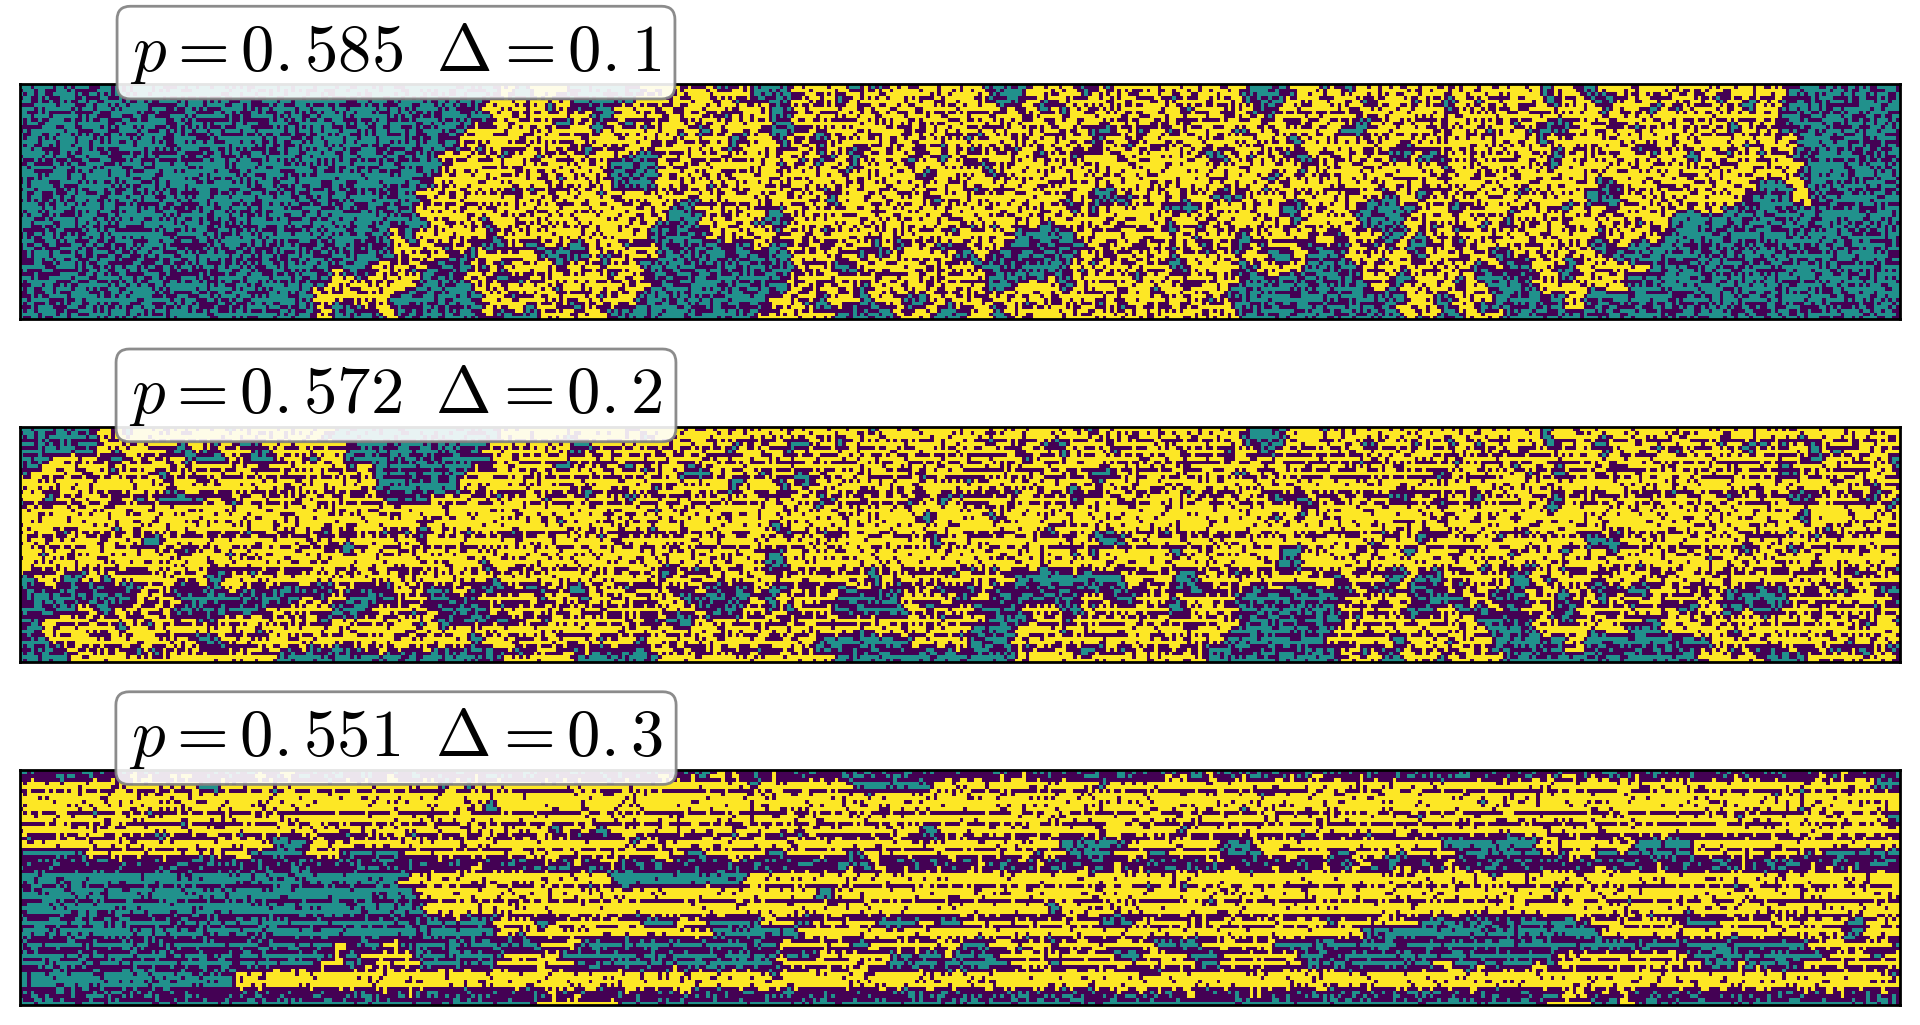
\includegraphics[width=\textwidth]{chapters/ch5-anis/figs/mlperco}
\end{center}
\caption{Three realizations of the multi-layered percolation model in the
    square lattice. Black sites are unoccupied, dark cyan sites are occupied
    and yellow sites are represent the largest cluster of the system. All
    three realizations are in the critical point. The larger the value of
    $\Delta$, the more anisotropic is the system, and the multi-layered
    structure of the system becomes more evident.}
\label{fig:mlperco}
\end{figure}


\begin{figure}
\begin{center}
    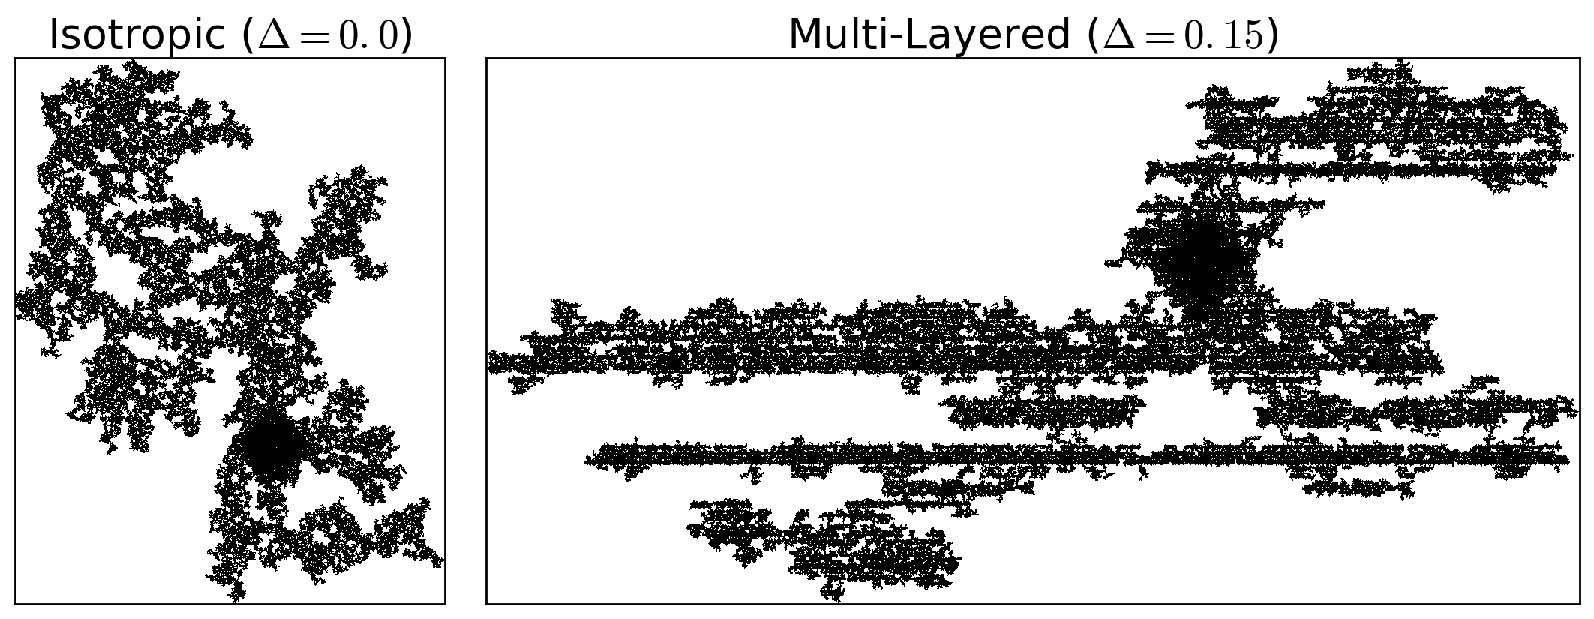
\includegraphics[width=\textwidth]{chapters/ch5-anis/figs/mlp_cluster}
\end{center}
\caption{A comparison of clusters of occupied sites in both isotropic and
    multi-layered percolation at their critical points. They were generated
    using the self-organized percolation algorithm~\cite{Parteli2010} (the
    dense ``core'' found on both clusters is an artifact of this method). The
    stratified nature of the multi-layered percolation makes itself evident
    even for the relatively low value of $\Delta$ used here.}
\label{fig:mlp_cluster}
\end{figure}

\begin{figure}
\begin{center}
    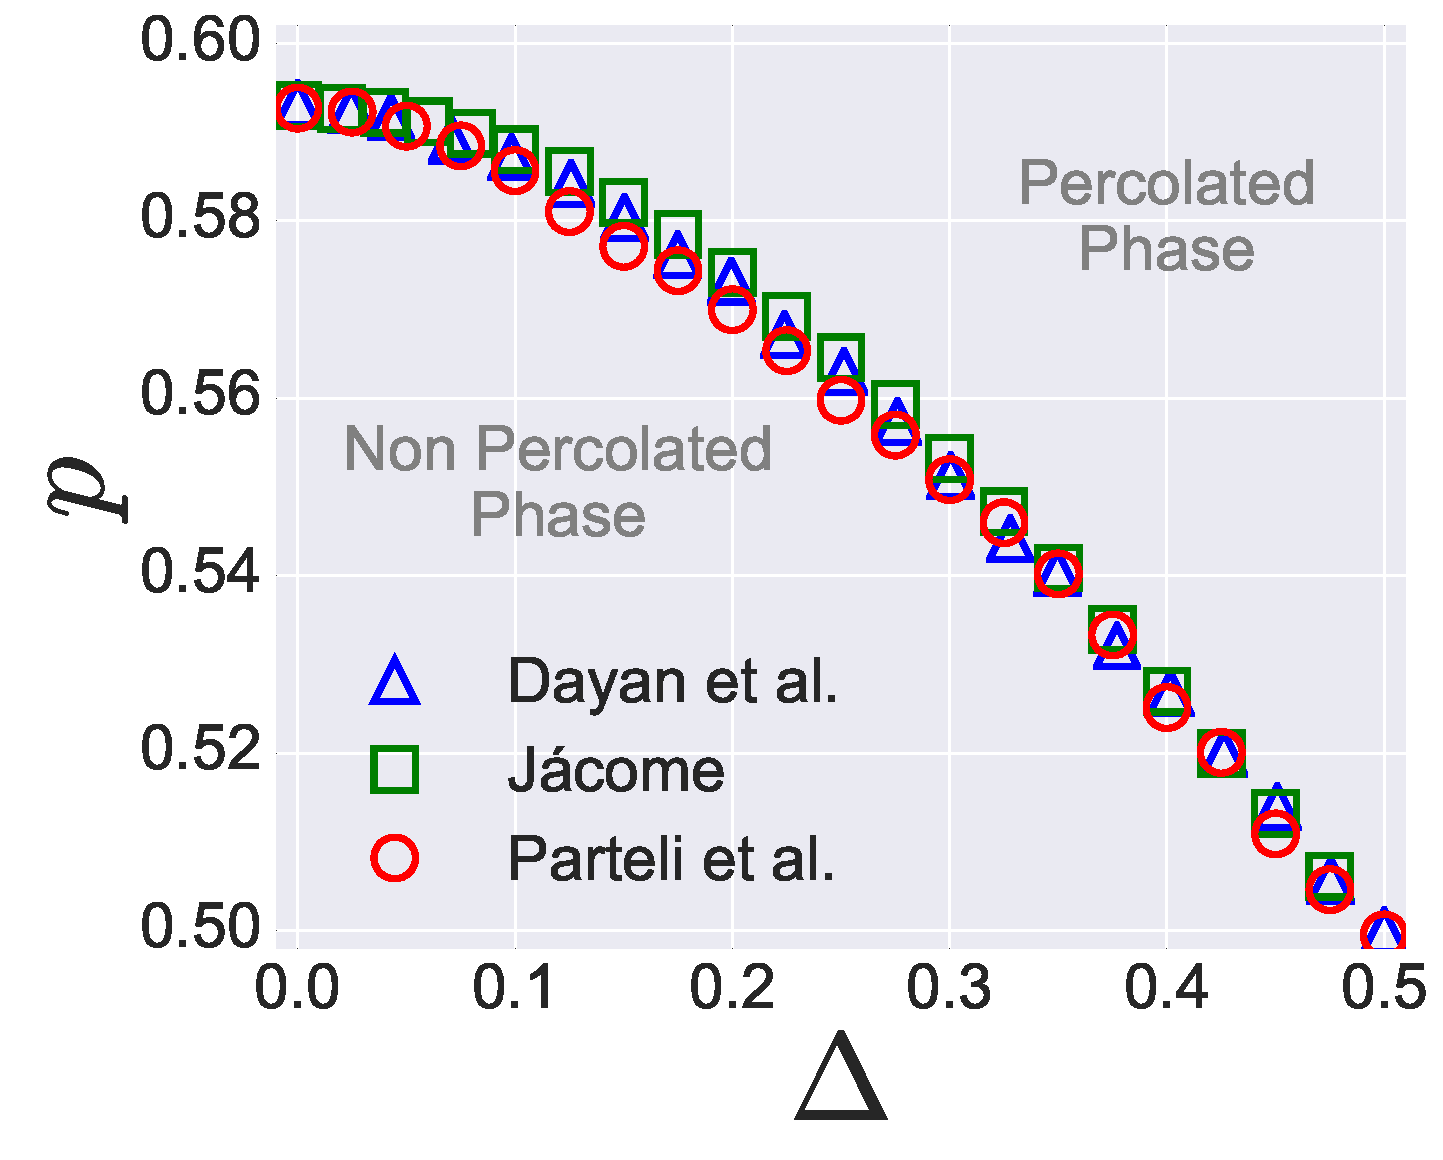
\includegraphics[scale=0.4]{chapters/ch5-anis/figs/mlp_ps0}
\end{center}
\caption{Phase diagram of the multi-layered percolation model on a square
    lattice showing the critical line separating the two phases computed in
    three different occasions by Dayan~\cite{Dayan1991},
    J\'acome~\cite{Samyr2009}, and Parteli~\cite{Parteli2010}. We observe that
    $p_c\approx0.592$ for for $\Delta=0$, which is the expected value for
    isotropic percolation.}
\label{fig:mlp_ps0}
\end{figure}


\subsection{Directed Percolation}
\label{sec:dp}

Another very important universality class of strongly anisotropic systems is
yet another variation of the percolation model. Called \textit{directed
percolation}, this model can be seen as a spreading process. Starting from
some initial condition, any occupied site can spread and occupy an adjacent
site along a preferential direction with probability $p$; spread is prohibited
in all other directions. Figure~\ref{fig:dperco_scheme} illustrate the process,
and Figure~\ref{fig:dperco} shows the process in the three regimes:
subcritical, critical and supercritical.

Directed percolation is part of a larger group called dynamical phase
transitions, where there is a strict order of cause and effect which allows one
to interpret the preferred direction as a temporal coordinate. In the case of
directed percolation, the configuration of occupied sites in each row is
strictly determined by the state of the previous row alone. Because of this,
directed percolation is also an absorbing phase transitions, where the system
can reach a state from which it cannot leave, as is happens when a row is left
completely unoccupied. Systems below the critical point are expected to always
reach the absorbing state. This can be seen by looking at the average
occupation at time $t$, namely $\left\langle N(t)\right\rangle$, which can be
seen in Figure~\ref{fig:dperco_nt}. For $p<p_c$ we have that
$\lim_{t\rightarrow\infty}\left\langle N(t)\right\rangle=0$. At the critical
point however, we find the scaling relation
\begin{equation}
    \left\langle N\left(t\right)\right\rangle \sim t^{\Theta},
    \,\,\,\,\,\,\,\,\,
    p=p_c
\end{equation}
with the universal exponent $\Theta\approx0.302$~\cite{Henkel2008}. So we can
define the order parameter as the probability that the system never reaches the
absorbing state. This probability is null for $p\leq p_c$ but grows
continuously towards unity, just like a second-order phase transition should.

Unlike isotropic percolation, directed percolation is not an exactly solved
model. Its critical exponents can only be determined through numerical methods
and field theoretical expansions. In the $(1+1)$-dimensional case the values
found were $\nu_\perp=26/15$ and $\nu_\parallel=79/72$~\cite{Hinrichsen2000}
(the rational forms are conjectured, but experimental values are very close
with errors in the order of $10^{-4}$). Furthermore Owczarek \textit{et
al.}~\cite{Owczarek1997} analyzed the cluster perimeters in a similar way
done with multi-layered percolation, finding consistent values of exponents,
including $\bar{\nu}_\perp\approx0.557(5)$ and
$\bar{\nu}_\parallel\approx0.879(4)$.

Experimental realizations of directed percolation are hard to come by as
critical exponents are notoriously difficult to measure. A illustrious success
was found in turbulent liquid crystal transitions. More recently, experiments
and simulations on fluid dynamics indicate that the transition from laminar to
turbulent flow also belongs to the same universality class~\cite{Lemoult2016}.

\begin{figure}
\begin{center}
    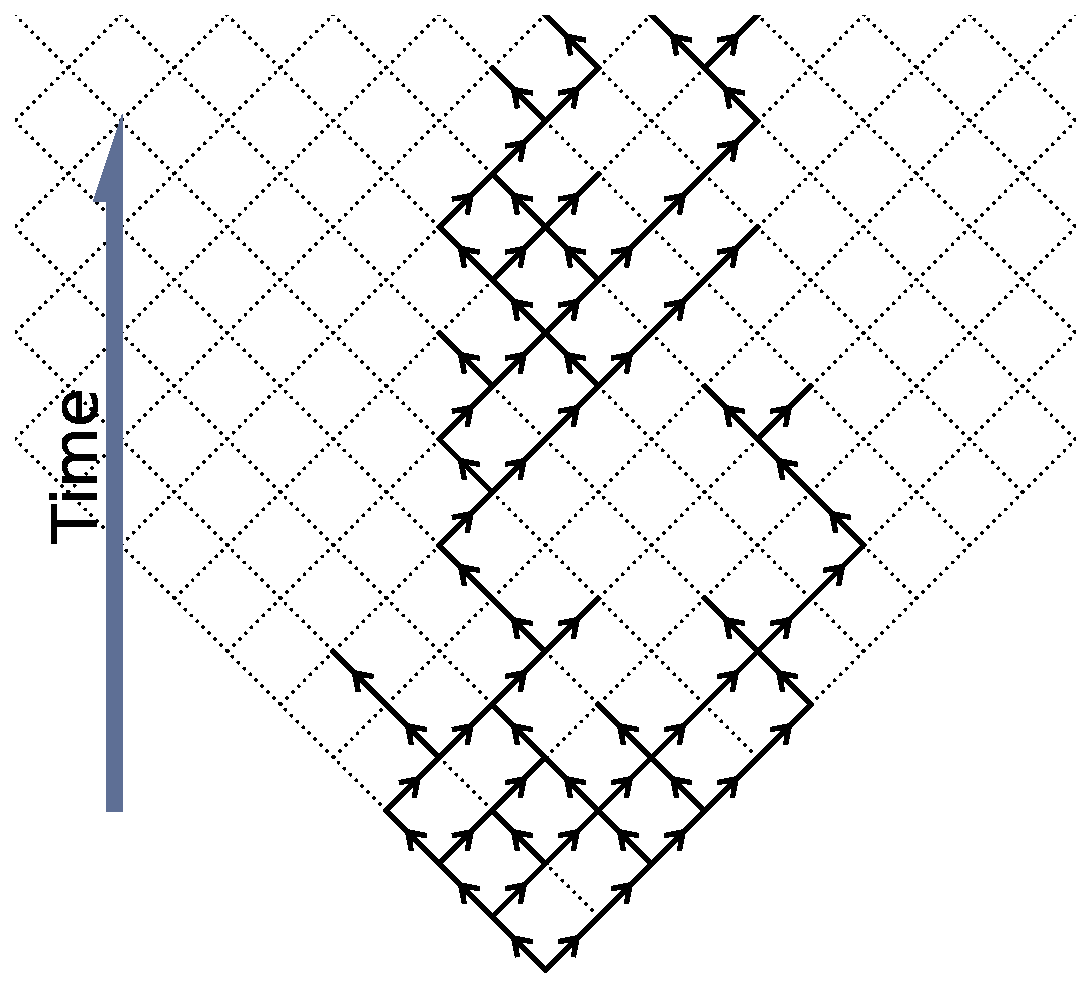
\includegraphics[scale=0.5]{chapters/ch5-anis/figs/dperco_scheme}
\end{center}
\caption{Simple representation of bond directed percolation in a square
    lattice. Here, the time flows upwards (although the time direction can be
    chosen arbitrarily). A previously occupied bond has a probability $p$ of
    occupying any of its two neighbors along the time direction.}
\label{fig:dperco_scheme}
\end{figure}

\begin{figure}
\begin{center}
    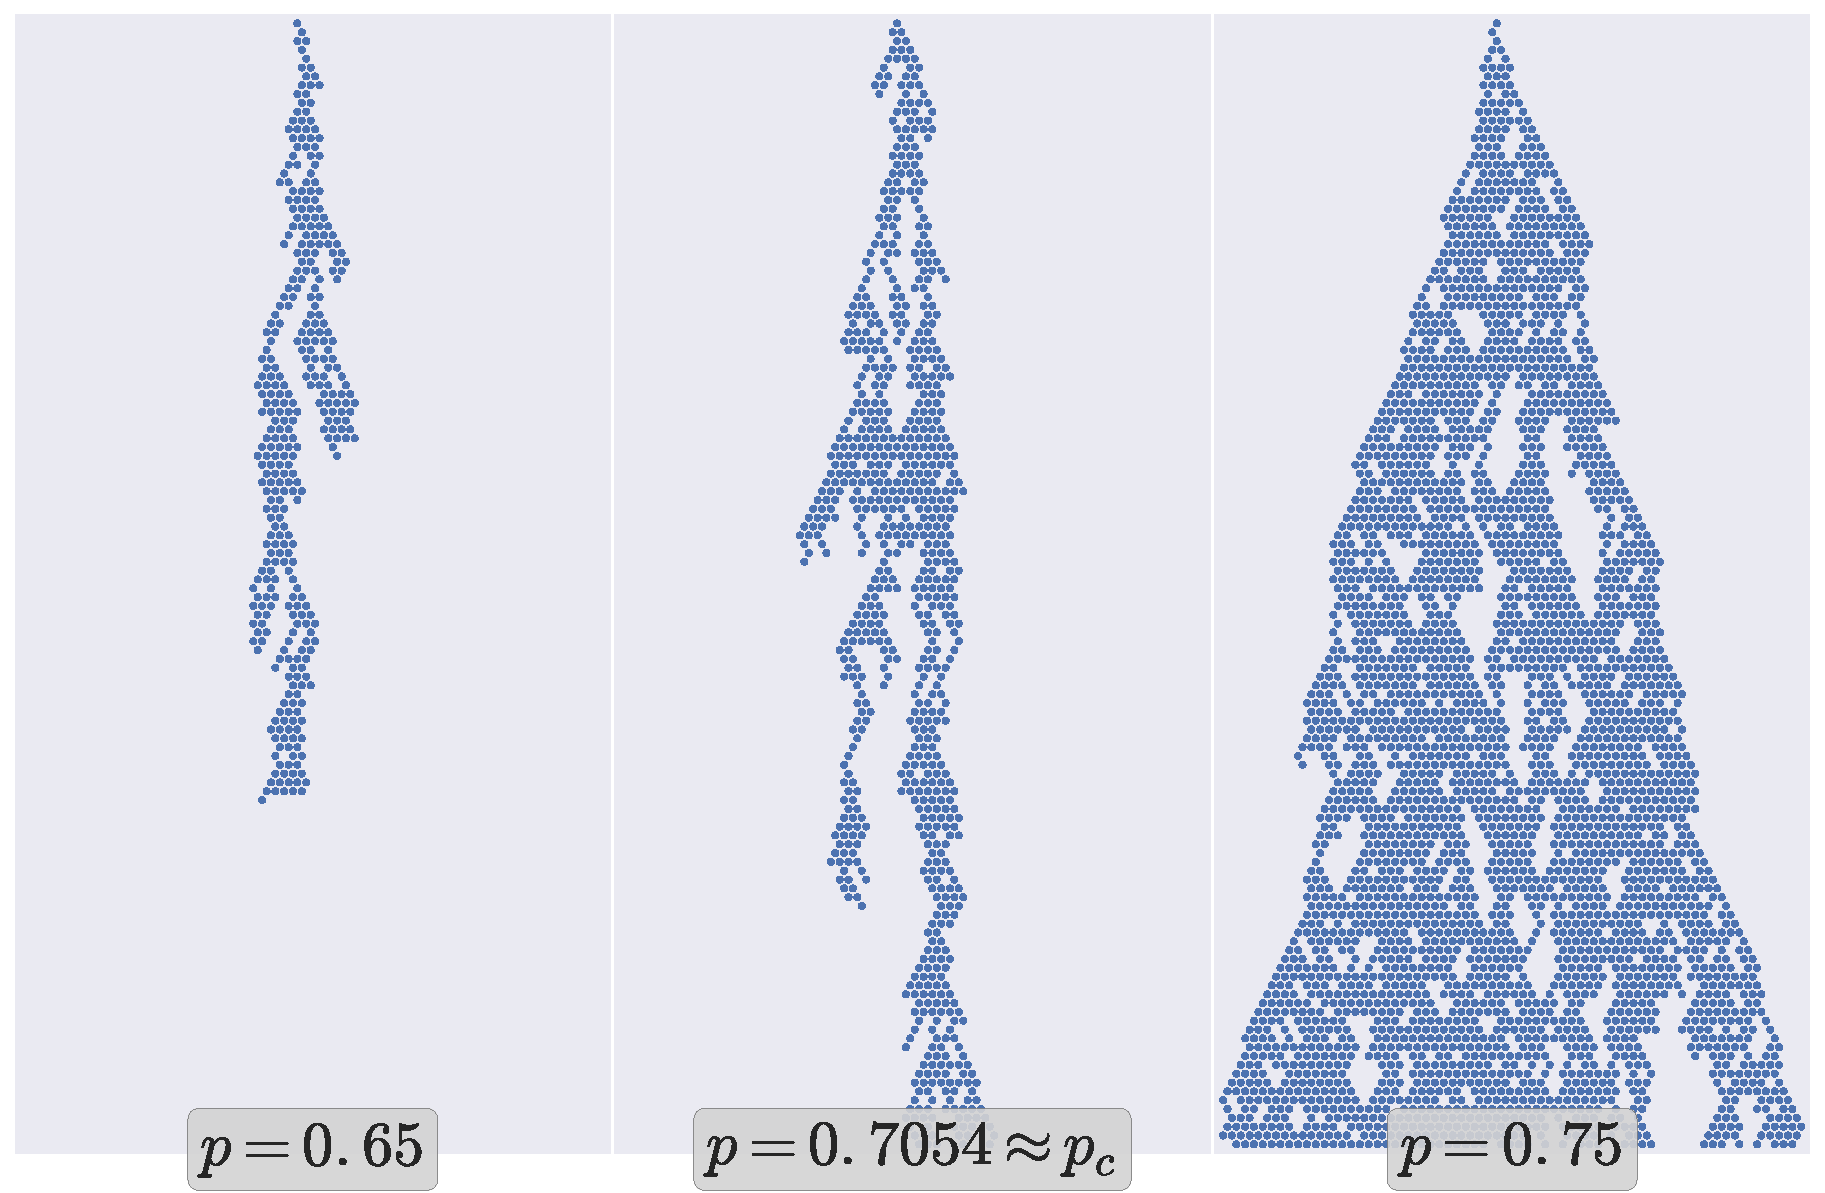
\includegraphics[scale=0.5]{chapters/ch5-anis/figs/dperco}
\end{center}
\caption{Three realizations of site directed percolation on a square lattice
    (here the time flows downwards). Being a absorbing phase transition model,
    the system have a probability of entering a state that it cannot leave, in
    this case a fully unoccupied state, like it happens in the left panel.
    Above the critical point however the probability of reaching an absorbing
    state becomes vanishing.}
\label{fig:dperco}
\end{figure}

\begin{figure}
\begin{center}
    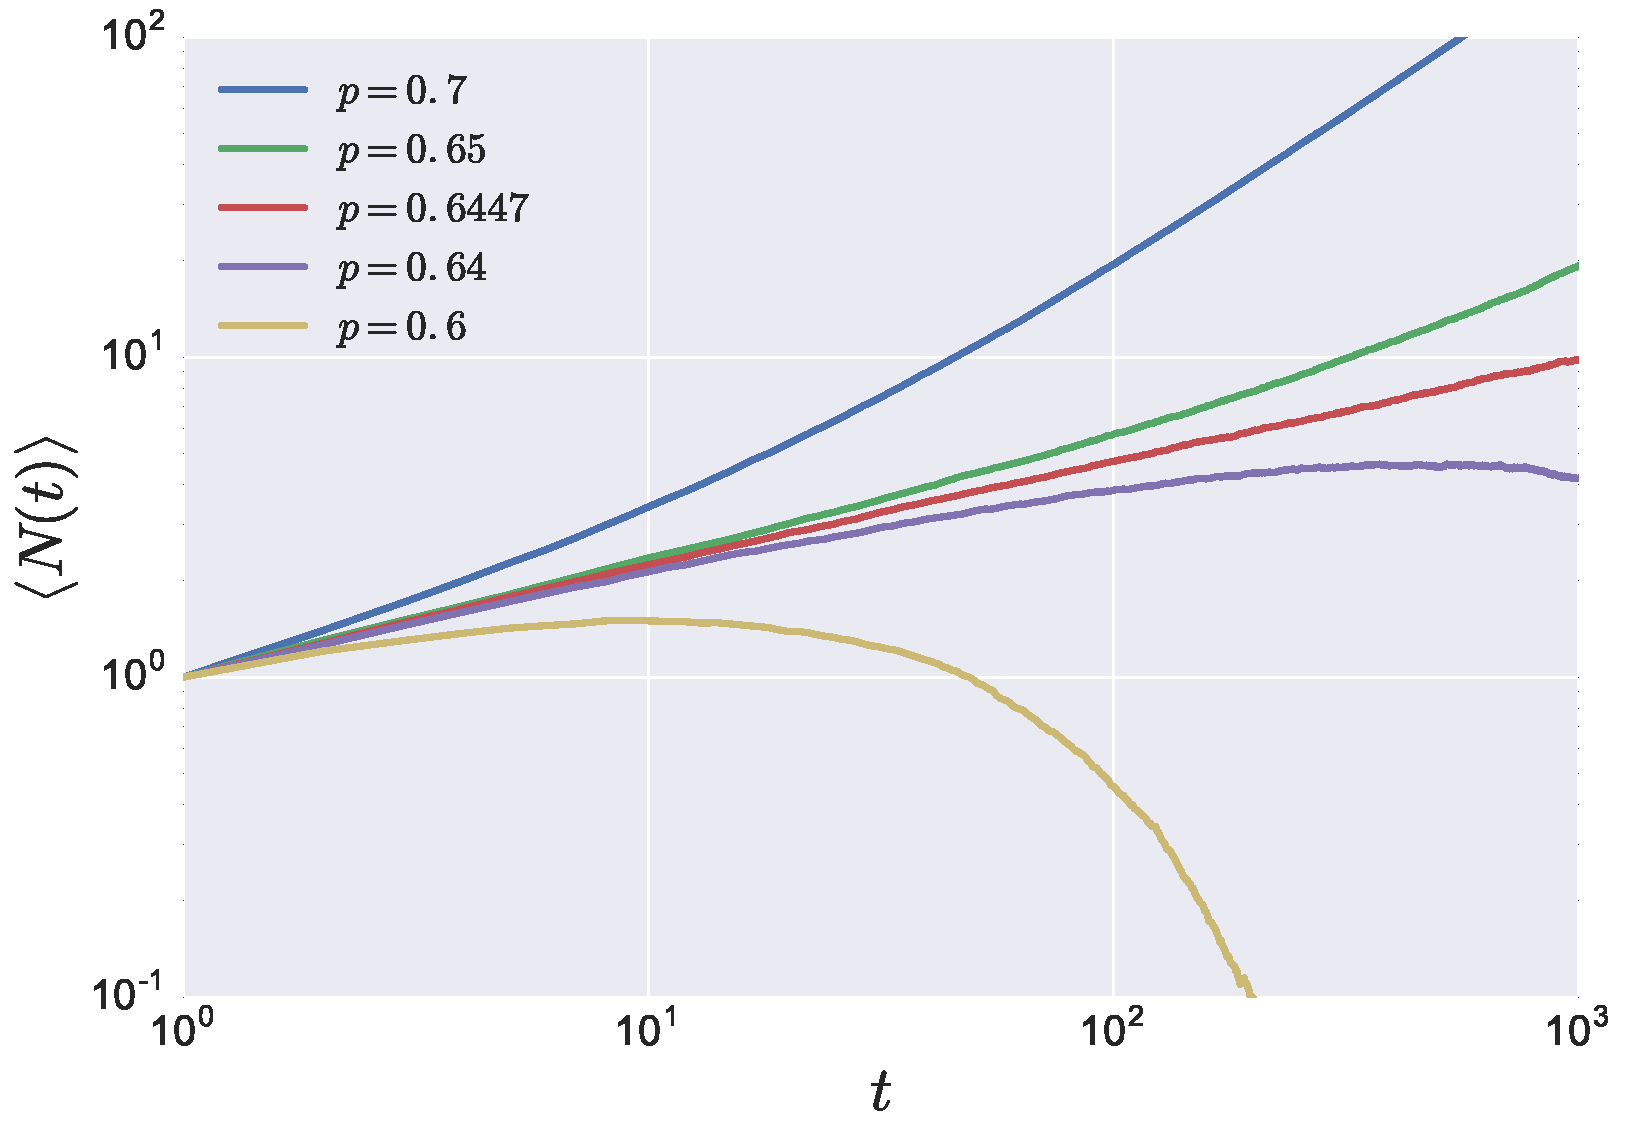
\includegraphics[scale=0.5]{chapters/ch5-anis/figs/dperco_nt}
\end{center}
\caption{Expected population of bond directed percolation as a function of time
    for various values of $p$. The critical point ($p_c\approx0.6447$) is the
    lowest value of $p$ such that $\lim_{t\rightarrow\infty}\left\langle
    N(t)\right\rangle>0$.}
\label{fig:dperco_nt}
\end{figure}
